\section{Evaluation}
\label{sec:evaluation}

\subsection{Ground Truth Construction}
\label{sec:ground-truth}

Relevance judgements were collected using TREC-style depth-20 pooling. For each of the 10 queries, the top-20 results from each of the three retrieval approaches were unioned and deduplicated, yielding 218 unique candidate frames. Each candidate was then manually assigned a binary relevance label, where 1 denotes a relevant frame and 0 denotes a non-relevant frame. The final ground-truth set contains 71 relevant frames distributed across all 10 queries.

\subsection{Precision@10 Results}
\label{sec:results}

Precision@10 (P@10) is defined as the fraction of the top-10 retrieved frames that are relevant:

\[
\mathrm{P@10} = \frac{\left|\{r \in \mathrm{top\mbox{-}10} : r \in \mathrm{GT}\}\right|}{10}
\]

Table~\ref{tab:precision} reports P@10 for all 10 queries across the three retrieval approaches. Mean P@10 scores are 0.070, 0.620, and 0.640 for Approaches A, B, and C respectively.

\begin{table}[H]
\centering
\small
\begin{tabular}{lccc}
\toprule
Query & A & B & C \\
\midrule
Q1 & 0.1 & 0.5 & \bestscore{0.6} \\
Q2 & 0.1 & \bestscore{0.9} & \bestscore{0.9} \\
Q3 & 0.0 & \bestscore{0.4} & \bestscore{0.4} \\
Q4 & 0.0 & \bestscore{1.0} & \bestscore{1.0} \\
Q5 & 0.0 & \bestscore{1.0} & \bestscore{1.0} \\
Q6 & 0.4 & \bestscore{0.9} & \bestscore{0.9} \\
Q7 & 0.0 & \bestscore{0.3} & \bestscore{0.3} \\
Q8 & 0.1 & \bestscore{1.0} & \bestscore{1.0} \\
Q9 & 0.0 & 0.1 & \bestscore{0.2} \\
Q10 & 0.0 & \bestscore{0.1} & \bestscore{0.1} \\
\midrule
Mean & 0.070 & 0.620 & \bestscore{0.640} \\
\bottomrule
\end{tabular}
\caption{Precision@10 per query and approach. Bold underlined values indicate the best score per row. A~=~BM25 sparse, B~=~\textbf{SigLIP2} visual, C~=~\fusionname.}
\label{tab:precision}
\end{table}

The interactive retrieval interface is shown in Figure~\ref{fig:streamlit-ui}.

\begin{figure}[H]
  \centering
  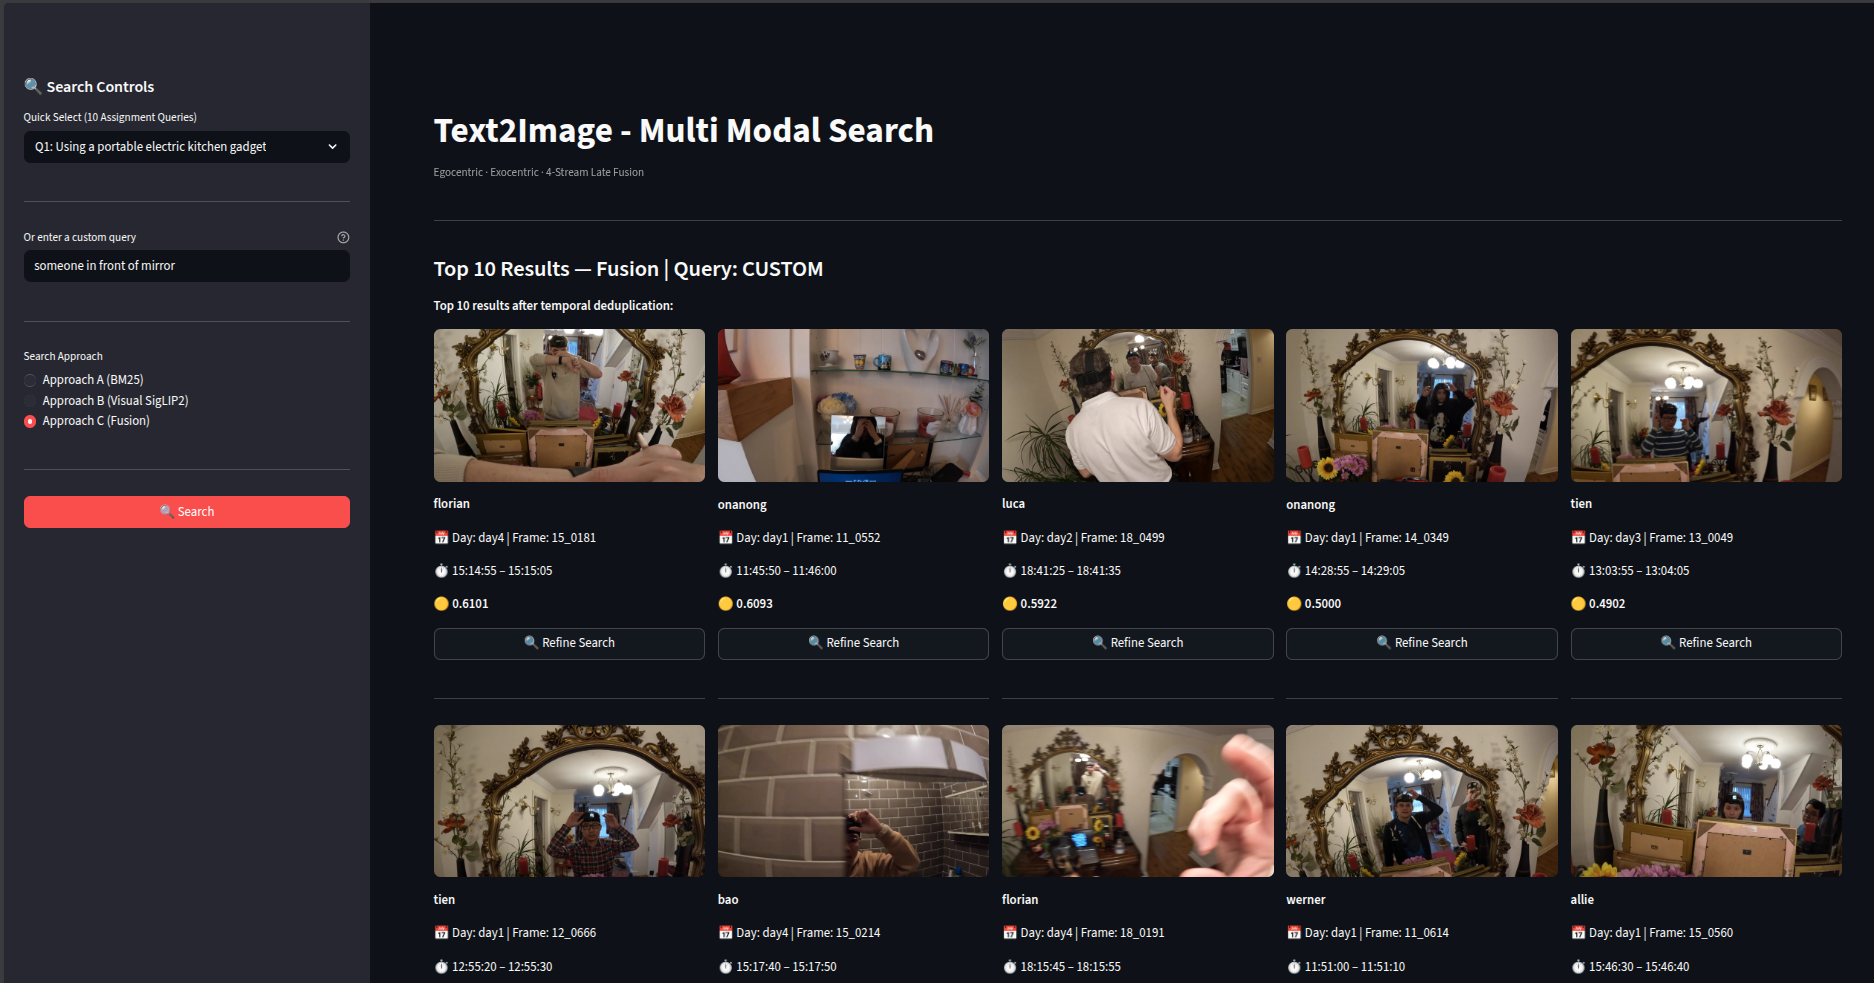
\includegraphics[width=\linewidth]{figures/streamlit_ui}
  \caption{Interactive Streamlit query interface showing top-10 retrieved frames, similarity scores, and approach selector for the MOS retrieval system.}
  \label{fig:streamlit-ui}
  \Description{Screenshot of the Streamlit search interface with query controls, approach selection, and a ranked grid of retrieved frames with scores.}
\end{figure}

\subsection{Analysis}
\label{sec:analysis}

Approach B substantially outperforms BM25 text retrieval, achieving a mean P@10 of 0.620 compared with 0.070 for Approach A. Activity queries Q4, Q5, and Q8 achieve perfect P@10 of 1.0 under Approach B, indicating that \textbf{SigLIP2} visual embeddings capture distinctive scene-level evidence more reliably than sparse transcript or caption text in this egocentric setting. This supports the central design decision of the system: when ASR is sparse or poorly aligned with frame content, dense visual embeddings become the dominant retrieval signal.

Approach C, implemented as \fusionname, ties or exceeds Approach B on 9 out of 10 queries and achieves the best overall mean P@10 of 0.640. Queries Q1 and Q9 each improve by 0.1 over the visual baseline, showing that caption and transcript evidence contributes complementary signal for activity-focused and symbol-recognition queries. No query falls below the Approach B baseline under fusion, indicating that the late-fusion and cross-encoder re-ranking stage improves precision without introducing regressions.

Approach A performs poorly as a standalone method, with a mean P@10 of 0.070 and non-zero scores only on Q1, Q2, Q6, and Q8. The limiting factor is modality mismatch: salient frame content is rarely described verbatim in co-occurring ASR transcripts, so keyword matching alone provides weak coverage for the lifelogging domain.

The OCR hallucination gate also had a measurable indexing impact. \textbf{Florence-2} hallucinated OCR text in 178,914 caption records, corresponding to 73.0\% of the 244,966-frame captioning corpus. The zero-shot \textbf{SigLIP2} cosine gate stripped all 178,914 records, yielding a 100\% removal rate. Retaining these ungrounded tokens would have injected systematic noise into both the \textbf{Whoosh} BM25 index and the \textbf{BGE-large-en-v1.5} caption embeddings, directly harming Approach A and the text component of Approach C.

\subsection{Failure Analysis}
\label{sec:failure}

Query Q7, which asks for a squirrel christmas tree ornament, remains challenging, with P@10 of 0.3 for both Approaches B and C. Global frame-level embeddings capture scene context more readily than fine-grained instance identity, so frames containing a christmas tree with multiple ornaments are compressed into a single representation that conflates several objects. A region-level grounding stage such as GroundingDINO \cite{liu2024groundingdino} would likely be necessary to localise the target ornament within cluttered scenes.

Query Q9, which asks for the ace of spades, shows a modest gain from fusion, with Approach C reaching 0.2 compared with 0.1 for Approach B. This improvement suggests that caption-derived context can help, but the query still depends on instance-level symbol recognition that remains below the semantic resolution of dense image-text embeddings trained on natural image-caption pairs.

Query Q10, which asks for a partially eaten apple, reaches only 0.1 under both Approaches B and C. The partially eaten state is a transient physical property that may produce only a weak change in a frame embedding relative to an intact apple. Detecting such state changes likely requires temporal reasoning over sequences rather than static frame-level retrieval.
